\chapter[Introdução]{Introdução}

%Este documento apresenta considerações gerais e preliminares relacionadas %à redação de relatórios de Projeto de Graduação da Faculdade UnB Gama (FGA). São abordados os diferentes aspectos sobre a estrutura do trabalho, uso de programas de auxilio a edição, tiragem de cópias, encadernação, etc.  

\par Atualmente, no Brasil, o número de cidadãos com algum tipo de deficiência chega aos 23.9\% da população total, sendo 7\% apenas pessoas com algum tipo de deficiência motora \cite{ibge2010}. Assim, é necessário criar formas de incluir tais pessoas, que uma vez inclusas podem ser uma grande parte da força econômica de um país. Pensando nisso, foram criadas leis para que ambientes públicos se adequassem para eliminar barreiras arquitetônicas às pessoas com deficiência [Leis N 10.048/2000 e N 10.098/2000] \cite{abnt2004}. Entretanto, isso não é suficiente para acabar com o problema de acessibilidade; é apenas um passo para a inclusão total desses indivíduos. Nesse contexto, torna-se necessária a criação de soluções criativas para que barreiras cada vez maiores sejam derrubadas. 
\par Um problema que muitos usuários de cadeira de rodas enfrentam é a falta de independência em ações básicas como fazer compras em um supermercado, dependendo muitas vezes de um acompanhante ou deslocamento para outro veículo propriedade do supermercado (ou \textit{scooters}). 

\par Dessa forma, o presente projeto busca sanar problemas relacionados à locomoção dentro do supermercado. A proposta é desenvolver um carrinho de compras autônomo que possa seguir uma pessoa com mobilidade reduzida. Assim, enquanto o cadeirante se desloca pelos corredores do supermercado, o carrinho será capaz de acompanhá-lo.
\par Haverá preocupação, igualmente, com o design da estrutura do carrinho. Será dado enfoque em dimensões apropriadas para cadeirantes, levando em consideração a distância que o carrinho de supermercado ficará do cadeirante quando este efetuar uma parada para colocar produtos nos compartimentos do carrinho.


\newpage



\section{Contribuição das engenharias}

Quanto às contribuições realizadas pela Engenharia de Energia, destacam-se:

\begin{\begin{itemize}
    \item Dimensionamentos dos motores e das baterias de modo a atender aos requisitos do carrinho, tais como o peso que este irá suportar e a respectiva potência que precisará; bem como o torque de partida do motor;
	\item Auxílio na confecção da estrutura, na própria usinagem e também em pesquisas quanto aos materiais que podem ser utilizados; 
	\item Desenvolvimento do carregador da bateria com a ajuda dos membros da Engenharia Eletrônica.
\end{itemize}

Quanto às contribuições da Engenharia Eletrônica, destacam-se:

\begin{itemize} 
    \item Localização do cadeirante, por meio de emissão/recepção de ondas eletromagnéticas
    \item Evitar todo e qualquer tipo de colisão a partir de algoritmos de controle de motor DC
    \item Projeto e fabricação de placas de circuito impresso de comunicação em Radio-frequência e Ponte H;
    \item Especificação de sensores de distância adequados.
\end{itemize}
 
Quanto às contribuições de Engenharia de Software, destacam-se:
\begin{itemize}
    \item Algoritmo de processamento de imagens em tempo real;
    \item Algoritmo de captura da distância através do sensor ultrassom;
    \item Algoritmo de controle dos motores integrado aos algoritmos supracitados;
    \item Aplicação da técnica PID para selecionar os melhores \textit{inputs} de distância.
    \item Utilização de questionário como técnica de identificação de requisitos;
    \item Especificação e documentação: definição de requisitos funcionais e não-funcionais;
    \item Representação gráfica dos algoritmos;
    \item Gerência de configuração de software:  identificação da configuração dos algoritmos com a finalidade de controlar mudanças e configurar o ambiente de desenvolvimento e de implantação.
\end{itemize}

Quanto às contribuições da Engenharia Automotiva, destacam-se:

\begin{itemize}
    \item Realização do projeto de estrutura e análise estrutural de forma analítica e numérica, verificando também a parte de transmissão de potência do motor para as rodinhas, de modo que o carrinho consiga se movimentar considerando o seu peso máximo;
    \item Fabricação da estrutura e de suas peças componentes, determinando o melhor material a ser utilizado, para garantir a resistência estrutural, o melhor processo de fabricação a ser utilizado e garantindo a integração de todos os componentes.
\end{itemize}

Quanto às contribuições da Engenharia Aeroespacial, destacam-se:

\begin{itemize}
    \item Auxiliar no projeto e construção da estrutura do carrinho;
    \item Realizar análise numérica bem como otimização da geometria e escolhendo melhor material a ser utilizado.
\end{itemize}


\section{Objetivo Geral}

O objetivo geral do projeto consiste em realizar a confecção de um carrinho de compras de supermercado autônomo. Assim,ele irá acompanhar o cadeirante sem que haja controle pelo usuário do serviço de forma eficiente e acessível, por meio de tecnologias específicas como sensoriamento

\section{Objetivos Específicos}

O projeto vigente tem como finalidades específicas:

\begin{itemize}  
\item Obter o produto com características ideais que cumpra os requisitos propostos para confecção do projeto;
\item Realizar o projeto com custos reduzidos;
\item Desenvolver algoritmo capaz de acompanhar o cadeirante;
\item Incorporar sensores para a detecção de possíveis obstáculos;
\item Estabelecer uma nova ergonomia para o carrinho de compras;
\item Integrar dispositivos tendo suas responsabilidades divididas por áreas das engenharias culminará no objetivo geral do projeto, descrito anteriormente;
\end{itemize}

\section{Estudo de viabilidade} \label{sec:estudo_viabilidade}

\par Para a realização do projeto foi aplicado um estudo piloto de forma a verificar a viabilidade do produto a ser desenvolvido e a definição de alguns requisitos do projeto. Com isto, foi realizado uma pesquisa para verificar e contextualizar a relevância do projeto  para aumentar a acessibilidade dos cadeirantes em supermercados  e a disponibilidade por parte dos representantes destes em implementar o produto.

\par A pesquisa foi dividida em dois formulários, sendo um exclusivo para cadeirantes e o outro para os representantes de supermercado. O primeiro formulário tem como objetivos:

\begin{itemize}  
\item Buscar as características do público alvo do projeto;
\item Identificar o volume das compras realizado por cadeirantes;
\item Identificar a dificuldade em realizar compras por parte dos cadeirantes;
\item Verificar a aceitação e o interesse do público alvo pelo projeto a ser implementado;
\item Levantar sugestões de aprimoramento do produto de acordo com a visão do público alvo;
\end{itemize}

\par O segundo formulário tem como objetivos:

\begin{itemize}  
\item Buscar as características do público alvo do projeto de acordo com a visão dos representantes de supermercado;
\item Identificar ferramentas de suporte aos cadeirantes já oferecidas pelos supermercados;
\item Verificar a aceitação e o interesse por parte dos supermercados em implementar o produto;
\item Identificar uma margem de custo na qual o supermercado estaria disposto a pagar pelo produto;
\end{itemize}

\par Para validar o objetivo do estudo o questionário foi implementado na plataforma \textit{Typeform}. Essa plataforma permite que os usuários respondam o questionário de forma virtual, tanto em computadores quanto com \textit{smartphones}, otimizando o processo da pesquisa. Foram feitas 18 perguntas, sendo 12 perguntas para o questionário voltado para os cadeirantes e 6 perguntas voltadas para os representantes  de supermercados. O resultado é apresentado na Tabela \ref{tab:quest_viabilidade}.

\begin{sidewaystable}[]
\centering
\caption{Resultado questionário do estudo de viabilidade. Fonte: Autores.}
\label{tab:quest_viabilidade}
\resizebox{\textwidth}{!}{%
\begin{tabular}{lll}
Pergunta                                                                               & Propósito                                                                                    & Resultados                                      \\
Sexo                                                                                   & Identificar o perfil dos respondentes                                                        & Masculino                                       \\
Idade                                                                                  & Identificar o perfil dos respondentes                                                        & 45 a 60 anos                                    \\
Qual o modelo da cadeira de rodas?                                                     & Buscar características do público alvo                                                       & Automatizada                                    \\
Possui veículo próprio?                                                                & Buscar características do público alvo                                                       & Não                                             \\
Faz compras no supermercado?                                                           & Buscar características e identificar o perfil do público alvo                                & Sim                                             \\
Realiza compras acompanhado(a)?                                                        & Buscar características e identificar o perfil do público alvo                                & Sempre/ ás vezes                                \\
Quanta vez no mês frequenta o supermercado?                                            & Buscar características e identificar o perfil do público alvo                                & Mais de 4 vezes                                 \\
Qual o volume de compras por cada ida ao supermercado?                                 & Identificar o volume das compras realizado por cadeirantes                                   & Médio                                           \\
Caso vá sozinho, o supermercado oferece algum serviço para auxiliá-lo?                 & Identificar a dificuldade em realizar compras por parte dos cadeirantes                      & Não                                             \\
Quais as principais dificuldades que encontra no supermercado?                         & Identificar a dificuldade em realizar compras por parte dos cadeirantes                      & Carregar as compras / Pegar itens na prateleira \\
Um carrinho autônomo você acha que pode auxiliar nesse processo?                       & Verificar a aceitação e o interesse do público alvo pelo projeto a ser implementado          & Sim                                             \\
Quais aspectos o carrinho autônomo deve oferecer?                                      & Levantar sugestões de aprimoramento do produto de acordo com a visão do público alvo         & Altura,Volume e Velocidade                      \\
Á frequente a presença de clientes cadeirantes no supermercado?                        & Buscar características e identificar o perfil do público alvo                                & Não / Sim (50\% pra cada)                       \\
Quais serviços de auxilio o supermercado oferece?                                      & Identificar ferramentas de suporte aos cadeirantes já oferecidas pelos supermercados         & Acessibilidade                                  \\
Seria interessante implementar carrinhos autônomos para auxiliar os cadeirantes?       & Verificar a aceitação e o interesse por parte dos supermercados em implementar o produto     & Sim                                             \\
O quanto o supermercado estaria disposto a pagar pelo produto?                         & Identificar uma margem de custo na qual o supermercado estaria disposto a pagar pelo produto & R\$ 500 a R\$ 1000                                \\
O supermercado acredita que o carrinho autônomo pode oferecer diferencial competitivo? & Verificar a aceitação e o interesse por parte dos supermercados em implementar o produto     & Sim                                             \\
Os cadeirantes que frequentam o supermercado vão sozinhos ou acompanhados por alguém?  & Buscar características e identificar o perfil do público alvo                                & Sozinhos                                       
\end{tabular}}
\end{sidewaystable}

%--------------------------------------------------------------------
%Requisitos



\chapter{Requisitos}
Como em qualquer projeto, seu desenvolvimento deve ser executado de acordo com uma sequência de requisitos fundamentais que devem ser seguidos. Dentre eles encontram-se os requisitos de funcionamento e desempenho, requisitos estatutários e regulamentares a serem aplicados e outros requisitos essenciais para projeto e desenvolvimento. Dessa forma, foram discutidos e definidos os requisitos. 


\section{Problemas mapeados}

Para o estabelecimento de requisitos completos e coesos com os objetivos da solução foi executado o estudo de viabilidade \ref{sec:estudo_viabilidade} que fomentou a criação do diagrama de causa e efeito (Figura \ref{fig:causa_e_efeito}). Os problemas foram categorizados em problemas de acesso, localização, carga e tempo.

\begin{figure}[hb]
		\centering
		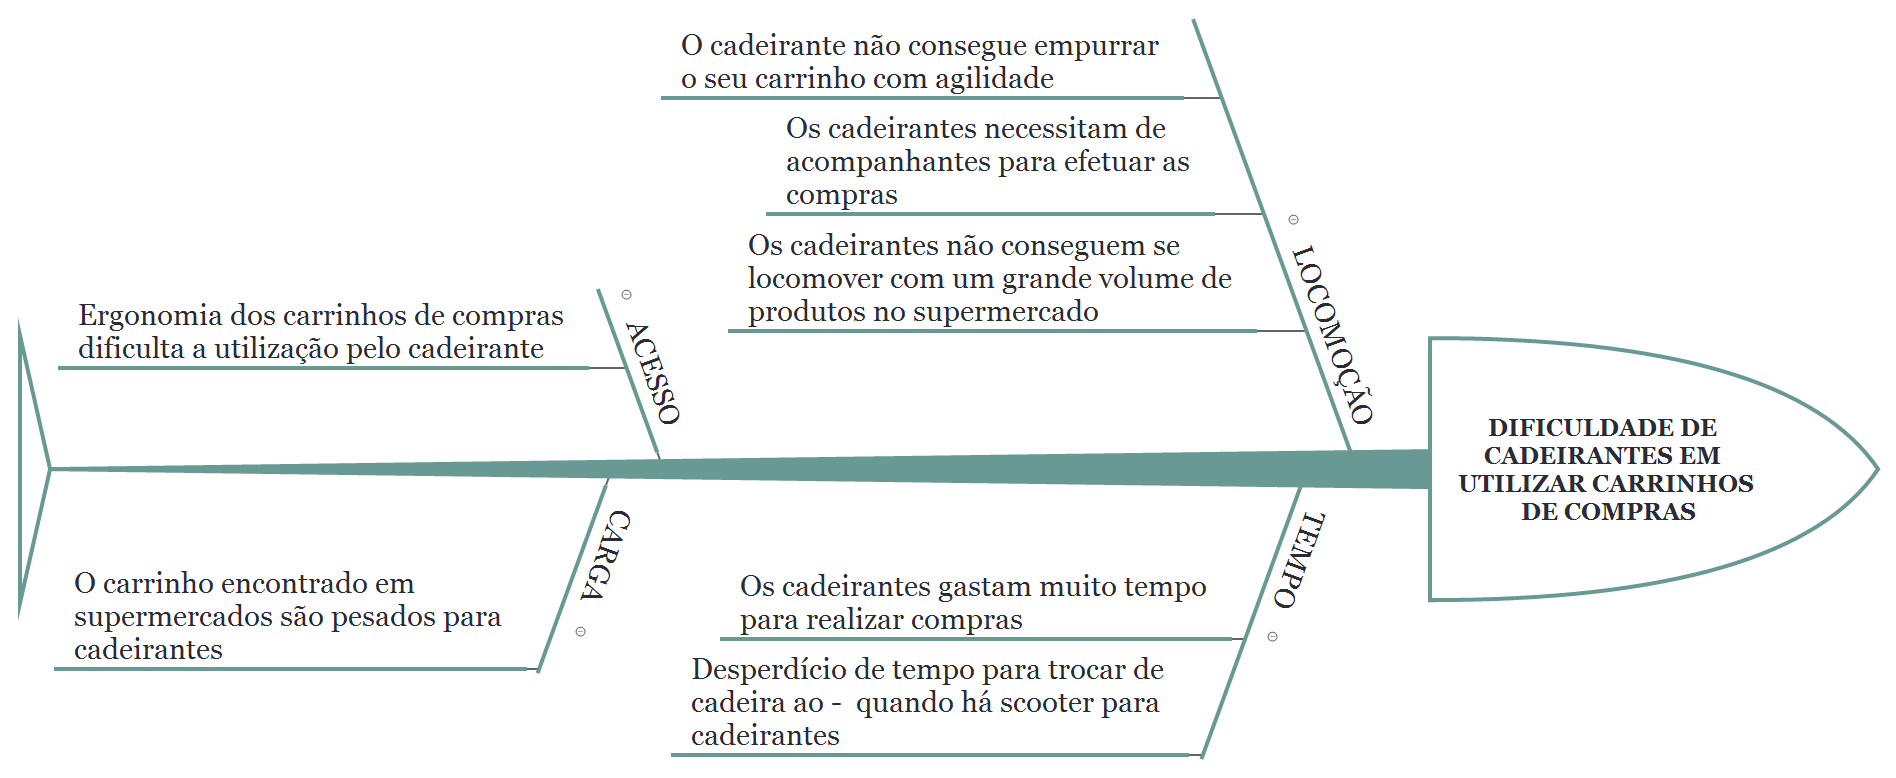
\includegraphics[width=1\textwidth]{figuras/diagramaefeito.png}
		\caption{Diagrama de Causa e Efeito. Fonte: Autores}
		\label{fig:causa_e_efeito}
\end{figure} 

\section{Requisitos funcionais}

A Tabela \ref{tab:req_func} apresenta os requisitos funcionais do produto e demonstra a dependência entre os mesmos além de promover a rastreabilidade dos problemas para a solução.  As categorias Locomoção, Acesso e Carga definidas pelo diagrama de causa e efeito são diretamente atacadas pelo requisito da solução. A categoria Tempo é indiretamente solucionada em todo o conjunto de requisitos.


% ######## init table ########
\begin{table}[h]
 \centering
 \caption{Requisitos funcionais do projeto} \label{tab:req_func}
% distancia entre a linha e o texto
 {\renewcommand\arraystretch{1.25}
 \begin{tabular}{ l l l l }
  \cline{1-1}\cline{2-2}\cline{3-3}\cline{4-4}  
    \multicolumn{1}{|p{3.167cm}|}{\textbf{Categoria de Problemas}} &
    \multicolumn{1}{p{1.283cm}|}{\textbf{Id }} &
    \multicolumn{1}{p{4.783cm}|}{ } &
    \multicolumn{1}{p{2.383cm}|}{\textbf{Dependência}}
  \\  
  \cline{1-1}\cline{2-2}\cline{3-3}\cline{4-4}  
    \multicolumn{1}{|p{3.167cm}|}{Locomoção} &
    \multicolumn{1}{p{1.283cm}|}{1} &
    \multicolumn{1}{p{4.783cm}|}{O carrinho deverá seguir o cadeirante de forma autônoma pelo supermercado considerando-se um ambiente ideal, ou seja, chão plano;} &
    \multicolumn{1}{p{2.383cm}|}{2, 3, 4}
  \\  
  \cline{1-1}\cline{2-2}\cline{3-3}\cline{4-4}  
    \multicolumn{1}{|p{3.167cm}|}{ } &
    \multicolumn{1}{p{1.283cm}|}{2} &
    \multicolumn{1}{p{4.783cm}|}{A distância entre o carrinho e o cadeirante será de 20 a 50cm;} &
    \multicolumn{1}{p{2.383cm}|}{3}
  \\  
  \cline{1-1}\cline{2-2}\cline{3-3}\cline{4-4}  
    \multicolumn{1}{|p{3.167cm}|}{ } &
    \multicolumn{1}{p{1.283cm}|}{3} &
    \multicolumn{1}{p{4.783cm}|}{O carrinho deverá ser capaz de desviar de obstáculos ao fazer curvas;} &
    \multicolumn{1}{p{2.383cm}|}{ }
  \\  
  \cline{1-1}\cline{2-2}\cline{3-3}\cline{4-4}  
    \multicolumn{1}{|p{3.167cm}|}{ } &
    \multicolumn{1}{p{1.283cm}|}{4} &
    \multicolumn{1}{p{4.783cm}|}{O cadeirante terá disponível um botão on/off para o carrinho;} &
    \multicolumn{1}{p{2.383cm}|}{ }
  \\  
  \cline{1-1}\cline{2-2}\cline{3-3}\cline{4-4}  
    \multicolumn{1}{|p{3.167cm}|}{Acesso} &
    \multicolumn{1}{p{1.283cm}|}{5} &
    \multicolumn{1}{p{4.783cm}|}{O carrinho deverá conter o espaço/estrutura necessária para o cadeirante colocar suas compras;} &
    \multicolumn{1}{p{2.383cm}|}{ }
  \\  
  \cline{1-1}\cline{2-2}\cline{3-3}\cline{4-4}  
    \multicolumn{1}{|p{3.167cm}|}{ } &
    \multicolumn{1}{p{1.283cm}|}{6} &
    \multicolumn{1}{p{4.783cm}|}{A estrutura do carrinho deve atender as medidas necessárias para o alcance do cadeirante} &
    \multicolumn{1}{p{2.383cm}|}{ }
  \\  
  \cline{1-1}\cline{2-2}\cline{3-3}\cline{4-4}  
    \multicolumn{1}{|p{3.167cm}|}{ } &
    \multicolumn{1}{p{1.283cm}|}{7} &
    \multicolumn{1}{p{4.783cm}|}{A posição do carrinho parado e/ou em movimento deve ser acessível ao cadeirante} &
    \multicolumn{1}{p{2.383cm}|}{3, 7}
  \\  
  \cline{1-1}\cline{2-2}\cline{3-3}\cline{4-4}  
    \multicolumn{1}{|p{3.167cm}|}{Carga} &
    \multicolumn{1}{p{1.283cm}|}{8} &
    \multicolumn{1}{p{4.783cm}|}{O carrinho terá um peso total de até 50kg, reservando-se 20kg para compras.} &
    \multicolumn{1}{p{2.383cm}|}{ }
  \\  
  \hline

 \end{tabular} }
\end{table}

\subsection{Requisitos não funcionais}

Os requisitos não funcionais definidos para a solução são listados abaixo:

\begin{itemize}
\item O carrinho terá velocidade máxima de 5km/h;
\item O carrinho terá autonomia de até 2 horas;
\item O carrinho deverá ser utilizado somente dentro do mercado, pelo cadeirante;
\item O carrinho poderá ser recarregável;
\item O carrinho será de propriedade do mercado, que o usará como adicional para necessidades especiais;
\item O cadeirante deverá ser instruído a andar devagar para que o carrinho consiga acompanhá-lo.
\end{itemize}


\subsection{Requisitos do projeto}

As restrições - e requisitos - do projeto são listados abaixo:

\begin{itemize}
\item O projeto do carrinho deverá conter detalhes de cada Engenharia em questão (Eletrônica, Software, Automotiva, Energia e Aeroespacial);
\item O projeto conterá três fases, sendo avaliadas em cada ponto de controle;
\item Na primeira fase deve ser apresentado o detalhamento da solução bem como os planos que regirão a condução do projeto;
\item Na segunda fase, serão apresentados os protótipos de cada subsistema funcionando.
\end{itemize}


